\documentclass{standalone}
\usepackage{tikz}
\usepackage{ctex,siunitx,ninecolors}
\setCJKmainfont{Noto Serif CJK SC}
\usepackage{tkz-euclide}
\usepackage{amsmath}
\usetikzlibrary{patterns, calc}
\usetikzlibrary {decorations.pathmorphing, decorations.pathreplacing, decorations.shapes,}
\begin{document}
\small
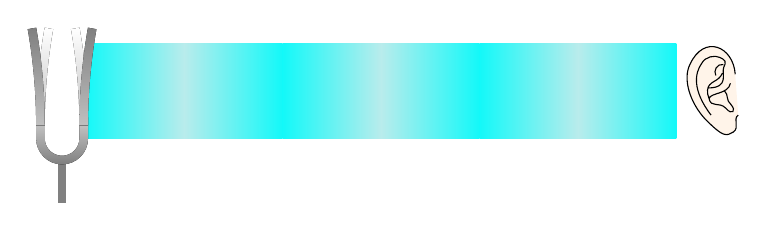
\begin{tikzpicture}[>=stealth, scale=1.0]
  % \useasboundingbox(-0.5,1.34)rectangle(7.55,-1.47);
  \foreach \x in {0.3,2.8,5.3}
  {
    \fill[left color=cyan!90!lightgray,right color=cyan!90!lightgray,middle color=cyan!40!lightgray!50](\x,0)rectangle++(2.5,1.2);
  }
  % \draw(0.3,0)rectangle(8,1.2);
  \begin{scope}[scale=0.55]
    \fill[gray](0.1,-0.45)rectangle(-0.1,-1.5);
    \fill[top color=lightgray,bottom color=gray](-0.4,0)arc(180:360:0.4)--++(0,0.3)--++(0.2,0)--++(0,-0.3)arc(0:-180:0.6)--++(0,0.3)--++(0.2,0)--cycle;
    \fill[bottom color=lightgray,top color=white](0.6,0.3)arc(0:10:13)--++(190:0.2)arc(10:0:12.8);
    \fill[bottom color=lightgray,top color=white](-0.4,0.3)arc(180:170:12.8)--++(170:0.2)arc(170:180:13);
    \fill[bottom color=lightgray,top color=gray](-0.4,0.3)arc(0:10:13)--++(190:0.2)arc(10:0:12.8);
    \fill[bottom color=lightgray,top color=gray](0.6,0.3)arc(180:170:12.8)--++(170:0.2)arc(170:180:13);
  \end{scope}
  \draw[fill=pink!20!orange!10](8.549,0.815)..controls(8.525,1.170)and(8.153,1.330)..
  (7.974,0.940)..controls(7.879,0.752)and(7.976,0.454)..
  (8.166,0.247)..controls(8.406,0.004)and(8.438,0.034)..
  (8.520,0.078)..controls(8.616,0.139)and(8.511,0.240)..(8.587,0.296);
  \draw 
  (8.242,0.296)..controls(7.999,0.615)and(8.034,0.831)..
  (8.125,0.956)..controls(8.169,1.039)and(8.289,1.062)..
  (8.354,1.028)..controls(8.424,0.997)and(8.440,0.976)..
  (8.402,0.899)..controls(8.374,0.827)and(8.477,0.644)..(8.209,0.641)
  (8.385,0.829)..controls(8.346,0.716)and(8.204,0.731)..
  (8.197,0.613)..controls(8.195,0.575)and(8.200,0.543)..
  (8.217,0.506)..controls(8.241,0.383)and(8.344,0.472)..
  (8.428,0.385)..controls(8.509,0.287)and(8.567,0.349)..
  (8.496,0.429)..controls(8.426,0.485)and(8.467,0.557)..(8.415,0.599)
  (8.217,0.506)..controls(8.234,0.583)and(8.460,0.558)..(8.488,0.700)
  (8.398,0.939)..controls(8.315,0.953)and(8.270,0.858)..(8.302,0.800); 

\end{tikzpicture}
\end{document}
